\chapter{Background Theory}
\label{chp:theory} 


\section{Robotic Maintenance of Industrial Installations}

\subsection{Introduction}

This project is a small part of a larger long-term goal concerning robotic maintenance. The goal of this section is to put the following background theory, and the implementation described in chapter \ref{chp:implementation}, into the context of the larger topic, which is automated robotic maintenance on industrial installations. It is important to describe how maintenance and inspection of industrial installations is done today, before application of robotic maintenance is discussed.  

\subsection{Potential Maintenance Tasks}

Hidden failure modes: PFD: What is the probability that a device (Fire detector, shut down valve, etc.) will fail when needed? 
Solution: Periodic maintenance.

\subsection{Offshore Installations}

\subsubsection{Corrosion}

Offshore installations are regularly, if not continuously exposed to harsh weather conditions in the form of wind and seawater. Presence of seawater, either through direct contact or in the form of drops and vapour, forms a very corrosive environment. In addition, the offshore environment is classified as the most corrosive environment in ISO 12944\cite{ElReedy2012383}. Common corrosion prevention methods are\cite{ElReedy2012383}:

\begin{itemize}
	\item Sacrificial Anodes.
	\item \ac{CP} in the form of a DC-current.
	\item Protective coating.
\end{itemize} 

In terms of maintenance, the sacrificial anodes can be subjected to periodic inspections and replacements, which could be done a robot. \ac{CP} can more easily be implemented with automated self tests, and should normally not require any inspections and maintenance\cite{ElReedy2012383}. Application of protective coating should ideally be applied in the controlled environment of a workshop. If protective coating is to be applied at sea, one should strive to make the conditions as favourable as possible.

\subsubsection{Fatigue}

Waves, wind, water currents and other forces subject offshore installations to structural stress.

\section{Robotic Maintenance Today}

Gas leak detection: \cite{FSR2014_gas_leak}. DARPA robotic challenge. Industrial ROS.

Today, robots outside of the R\&D laboratories and universities are usually put to perform a very limited set of specific tasks. Modern robots outperform humans in specific, repetitive and tedious tasks in controlled environments. For robotics in uncontrolled environments, there are still much research and development to be done. Several recent research papers(CITE en HAUG MED PAPERS!) indicate that significant advances are being made in the labs universities around the globe. Nevertheless, it is still some time before industrial robots will expand beyond repetitive and tedious tasks in controlled environments on on a large scale\cite{ifr_statistics}. A notable trend, and a step in the direction of uncontrolled environments, is increased human-robot collaboration\cite{cobotsEurope}.

A multitude of organizations and agents, e.g. \textit{ROS - Industrial}\cite{ROS_industrial}, Springer with the Springer Tracts in Advanced Robotics as well as the DARPA Robotics Challenge (DRC)\cite{DRC}, aims to incite innovation and progress related to industrial robotics and uncontrolled environments. 

 through competition, information flow and collaboration.

 that could probe useful in robotic maintenance are being developed a
 
The typical pre-programmed assembly robots still dominate the robotic market. They are usually found in manufacturing plants and large scale production\cite{ifr_statistics}, e.g. the automotive industry, where they perform dull, tedious tasks much faster and with higher accuracy than people. A notable trend in modern robotics is increased human-robot collaboration\cite{cobotsEurope}. Many new robots are being build for the human workspace, both in terms of safety and collaborative functionality. This trend is a step along the way of moving robots out of the controlled environment of a factory floor, and into the real world where a high degree of autonomy is required.

A report by a market research firm\cite{metraMartechGorle}, referenced to by \ac{IFR}\footnote{http://www.ifr.org/robots-create-jobs/}, points to three areas with potential for robotic applications:

\begin{itemize}
	\item Dangerous jobs, e.g. handling dangerous materials or work in high risk environments.
	\item Jobs that are economically infeasable in a high wage economy.
	\item Work which is impossible or highly infeasable for humans, e.g. space exploration, subsea maintenance or assembly of heavy components.
\end{itemize}

All of these factors motivate the development of robots for autonomous robotic maintenance.

There are particularily two fields \cite{subseaAIV}

\section{Modelling and Simulation}

\subsection{Some Terminology}

\subsubsection{Coordinate Systems and Poses}

\subsubsection{Robot Joints}

All links are connected to each other by joints. 

Coordinate systems are essential in the field of robotics. 

\subsection{Robot Modelling}

\subsection{Simulating in Gazebo}

\section{ROS}

\subsection{Introduction}

The \ac{ROS} is a collection of software libraries, tools and drivers intended for robot software development. A \ac{ROS} installation can be taylored to meet the demands of a wide range of robots with variyng complexity. \ac{ROS} is usually installed in the form of an already built Debian-package. These packages are only compatible with a few versions of Ubuntu which are specified on the \ac{ROS} homepage. When installed and configured, \ac{ROS} will run on top of Linux, and can be percieved as and extention of Linux itself. Installing \ac{ROS} from source is possible, but not recomended \cite{ROS_install}.

Roots of \ac{ROS} can be traced back to Stanford University at the beginning of the 2000s. At Stanford, several robotics software frameworks, including \ac{STAIR} and the \ac{PR} program, were created to provide dynamic, flexible and well tested foundations for further robot development and research. In 2007, a nearby start-up company and robot incubator, Willow Garage, sought to build upon these concepts, and initiated a collaborative and open development process of a new software framework. This framework eventually became \ac{ROS}\cite{ROS_history}\cite{rosbook15}. The framework can be used under the BSD open-source license, which means that ...\cite{BCD_license} Today, \ac{ROS} comes in many forms and comprise hundreds of advanced packages, algorithms and drivers, making it applicable for hobbyists, industrial automation, research and everything in between. 

\subsection{Important ROS Concepts}

The following descriptions are included in order to provide a complete, self-contained description of the project implementation. Similar descriptions can be found on the official \ac{ROS} website (INSERT LINK HERE), as well as in any book on \ac{ROS} (for example \cite{rosbook15}). 

\subsubsection{The ROS Graph}

A \ac{ROS} system comprise a set of small programs that communicate with each other. 

\subsubsection{roscore}

The \textit{roscore} is an essensial part of any \ac{ROS} system. It enables nodes to communicate with each other.

\subsubsection{Topics}

\subsubsection{Services}

\subsubsection{rosbridge}

\subsubsection{title}

\subsection{ROS-Related Tools}

\subsubsection{Robot Modelling In URDF}

\subsubsection{Visialization in RVIZ}

\subsubsection{Simulation in Gazebo}

\subsection{Structure of a ROS Application}

\subsection{Notable Robots Running ROS}

\paragraph{PR2 - Personal Robot 2}

PR2 is one of the first robots designed to run \ac{ROS} \cite{rosbook15}, and also one of the most advanced and capable robots with \ac{ROS} today. 

\paragraph{TurtleBot} 

The TurtleBot is a cheaper ROS-ready alternative to the PR2. 

\paragraph{Robonaut 2}

Robonaut 2, a dexterous humanoid robot, currently resides within the \ac{ISS} 400 km above the earth's surface. In 2014, a SpaceX Dracon capsule brought \ac{ROS} as well as a pair of legs for Robonaut up to the \ac{ISS}\cite{http://www.ros.org/news/2014/09/ros-running-on-iss.html}. Robonaut is designed for research on human-robot collaboration in space, and human-like tasks. For more information, follow \href{https://vimeo.com/106993914}{\textbf{this link}}\footnote{https://vimeo.com/106993914} to a talk on \ac{ROS} in space from ROSCon 2014.

Being the first robot with \ac{ROS} to be launched into space, 

\paragraph{Example of an industrial robot with ROS goes here!}

TODO!!!!!!!!!!

\section{Software}

\subsection{Qt}

\subsection{PCL}

\section{The Kinect Sensor}

\section{Software Tools}

\subsection{Point Cloud Library}

\subsection{ROS}

\subsection{Qt}


\subsection{Current Research and Applications}

\section{Introduction to Sensors in Autonomous Robots}

\subsection{Depth Cameras}

\subsubsection{Different Methods for Depth Perception}

In the context of this thesis, a depth camera is considered to be a sensor which the functionality of a regular video camera 

A depth camera can be described as a regular color video camera with the ability to create spatial images. In the context of this thesis, a depth camera can  more precisely be described as a RGB-D camera, which is short for red, green, blue and depth camera. A regular RGB camera will project a spatial scene onto a rectangular pixel grid, where each pixel contains intensity values for red, green and blue colors. These pixel values represents the detected scene. A major problem with RGB cameras is the significant loss of information. The information loss is mostly a consequence of 3d to 2d projection and digital quantization. RGB-D cameras have the means to reduce this information loss by mapping the pixel values to spatial coordinates, turning each pixel into voxels and the image into a point cloud of voxels. 

Different variations of depth cameras will usually fall into one of two categories: active or passive. Passive sensors perceive the surroundings as it is, without actively interfering with the environment as a part of the sensing process. A typical passive RGB-D sensor is the stereo camera. Stereo cameras use a stream of synchronized image pairs to perceive depth. The image pairs are displaced along the horizontal axis, and the depth information is extracted by searching for mutual information in the image pairs. How far the information is displaced from the left to the right image is directly related to how far away from the camera the information source is located. 

Active sensors depend on some form of projection onto the surroundings. For depth cameras, the projection is usually in the form of laser or infra red light. In RGB-D cameras it is essential that the projected light is distinguishable from the visible spectrum. The Kinect sensor used in this project is an example of an active RGB-D sensor. A proper introduction to the Kinect, will follow shortly.

\subsubsection{Natural User Interfaces - Origin of the Kinect}

\textbf{Forslag 1:}
When a group of designers are developing a new \ac{GUI}, they will often use a conceptual model when planning their design. The conceptual model is the mental model the designers want to put into the head of the user. All users will develop their own individual mental model, which is their high level understanding of how the \ac{GUI} works. A conceptual model may contain metaphors for things  the user already is familiar with. A painting program for example may use a metaphor for a canvas, paint brushes and palettes. When the mouse icon changes to a paint brush, most users will have an intuitive understanding of what it can do and how it is used. A \ac{NUI} will seek to remove the metaphors and create a more seamless interaction between the user and the machine. Some \ac{NUI}s may allow a user to write text with a pen instead of a keyboard, or dictate a letter with their voice while the computer converts audio into text. 

\textbf{Forslag 2:}
The idea behind a \ac{NUI} is to make \ac{HMI} as seamless and natural as possible. A \ac{NUI} allows the user to communicate without tools such as a keyboard or a mouse. From starting as ideas, science fiction and rare research projects, \ac{NUI}s can now be considered to be ubiquitous. Today, the most common form of \ac{NUI}s is the touch screen found in smart phones and tablets. 

The Microsoft Kinect sensor was initially designed as a \ac{NUI} for the Xbox 360 gaming console. The sensor allows users to use gestures and sounds to play console games. Later on, Microsoft has released SDKs, enabling developers to create \ac{NUI} applications for for Windows. 

The modern RGB-D sensors which are commonly used in robot research projects today were initially intended as \ac{NUI}.

\subsubsection{Kinect for Xbox 360}

Kinect for Xbox 360 is the RGB-D sensor used in this project. The device was initially intended as a \ac{NUI} for gaming and office applications. Possible use cases were inspired by early \ac{NUI} research at \ac{MIT} and, later on, the science fiction movie Minority Report, where Tom Cruice interacts with a computer by using hand gestures \cite{kinect_book}. The Kinect sensor is equipped with a depth sensor, a regular color camera, a microphone array and a tilt motor. The color camera in combination with the depth sensor forms what is usually referred to as a rgb-d sensor, i.e. a combined color and depth camera. This feature, combined with the relaticely low cost and accessability of the sensor as contributed to make the Kinect a very popular in research projects related to \ac{SLAM} and robotics.

Today, the the Kinect for Xbox 360 has been succeded by the Kinect for Xbox One, and is now considered to be a legacy device. Those considering to use the legacy Kinect should be aware of that it is becoming increasingly difficult, if not already impossible, to get hold of a new Kinect for Xbox 360. 

\begin{figure}[p]
    \centering
    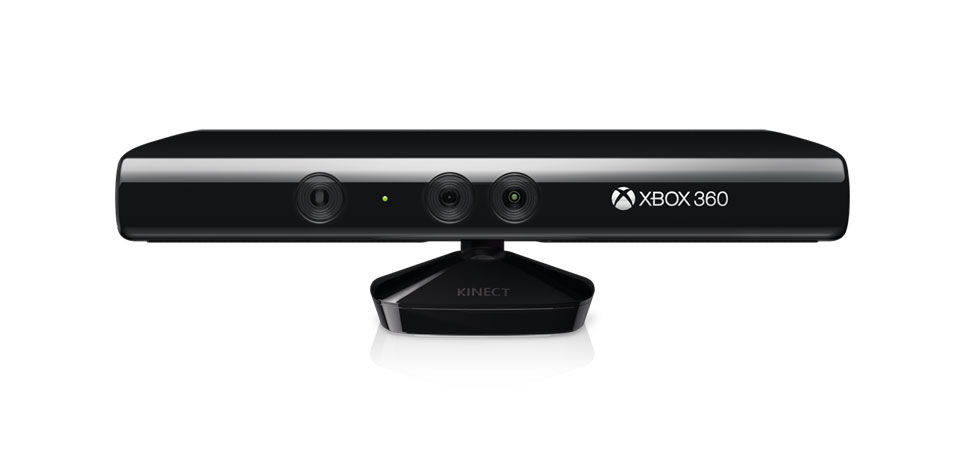
\includegraphics[width=0.8\textwidth]{kinect360}
    \caption{Awesome Image}
    \label{fig:kinect360}
\end{figure}

\begin{figure}[p]
    \centering
    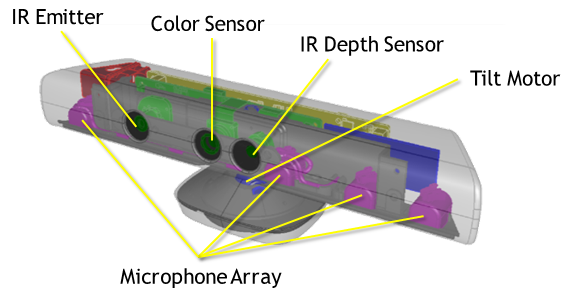
\includegraphics[width=0.8\textwidth]{kinect360_exp}
    \caption{Awesome Image}
    \label{fig:kinect360_exp}
\end{figure}


\subsection{Plannar Laser Sensors (LIDAR)}

A plannar laser sensor, also known as e.g. laser proximity sensors or laser radars, can all be referred to as LIDARs. 

\subsubsection{Scanning Laser Range Finder, URG-04LX-UG01}


\subsection{Odometers}

\subsection{Sensor Fusion}


\section{RTAB-Map}

\ac{RTAB-map} \cite{RTAB_map}.